\chapter{Resultados e discussões}
\label{cha:conclusoes}

Após todos os passos serem seguidos e os servidores devidamente configurados,
iniciaram-se os testes do \emph{OpenStack} para avaliar sua facilidade de uso,
performance e funcionalidades, colocando em julgamento também integração
com ferramentas para maiores abstrações (PaaS e SaaS) e o ciclo de desenvolvimento
do projeto.

\begin{figure}[h]
  \center
  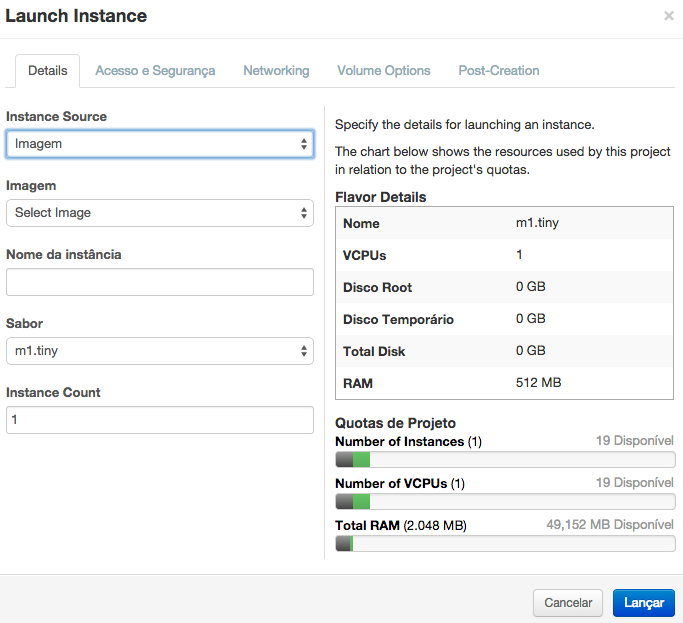
\includegraphics[scale=0.4]{imagem/criar-instancia-detalhes.png}
  \caption{Detalhes da nova instância a ser criada}
  \label{img:criar-instancia-detalhes}
  \center
  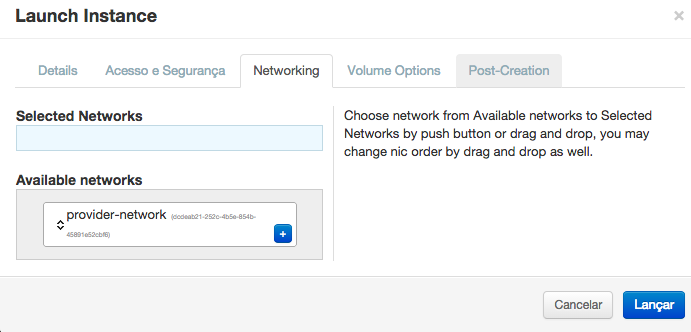
\includegraphics[scale=0.4]{imagem/criar-instancia-redes.png}
  \caption{Configurações de rede de uma nova instância}
  \label{img:criar-instancia-redes}
\end{figure}

A interface \emph{web} para gerenciamento das máquinas virtuais é extremamente simples,
desde a criação até a alteração dos recursos computacionais destas, atingindo
as expectativas com relação a este quesito. É possível definir vários ``sabores'' de máquinas
virtuais com configurações fixas de processador, armazenamento, memória e rede
(vide Figuras \ref{img:criar-instancia-detalhes} e \ref{img:criar-instancia-redes}).
Estas máquinas são criadas baseadas em imagens enviadas para o sistema e podem
ser ligadas e volumes persistentes de armazenamento para compartilhamento e
consolidação (agrupamento) de dados, como mostra a Figura \ref{img:criar-instancia-volume-site}.
Há também a  possibilidade de fazer um \emph{snapshot} (imagem) de um determinado servidor
para posterior restauração ou duplicação, criando outro servidores a partir deste
mesmo \emph{snapshot} (ver Figura \ref{img:imagens-e-snapshots}).

\begin{figure}[h]
  \center
  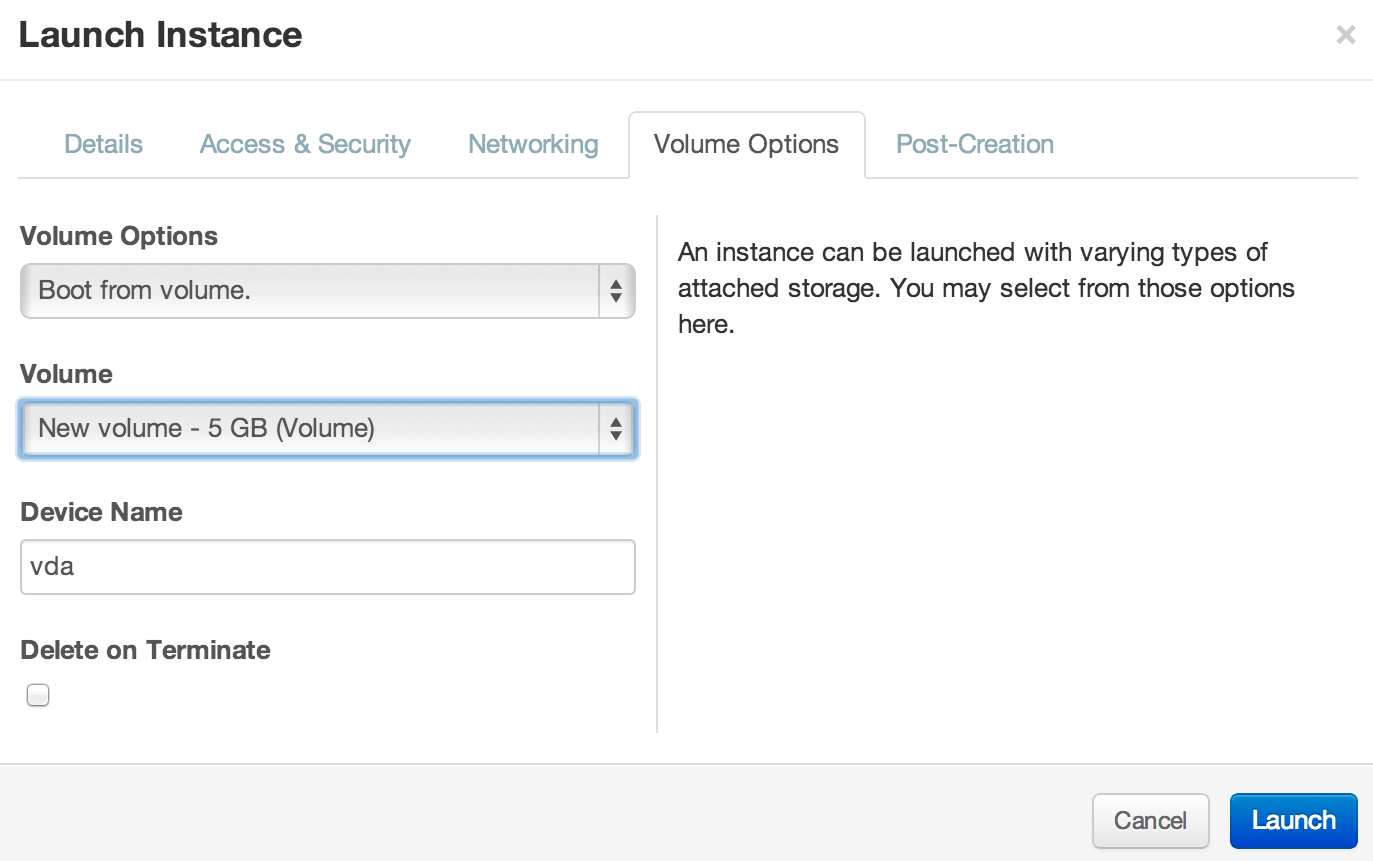
\includegraphics[scale=0.50]{imagem/criar-instancia-volume-site.png}
  \caption{Configurações de volume da nova instância}
  \label{img:criar-instancia-volume-site}
\end{figure}

\begin{figure}[h]
  \center
  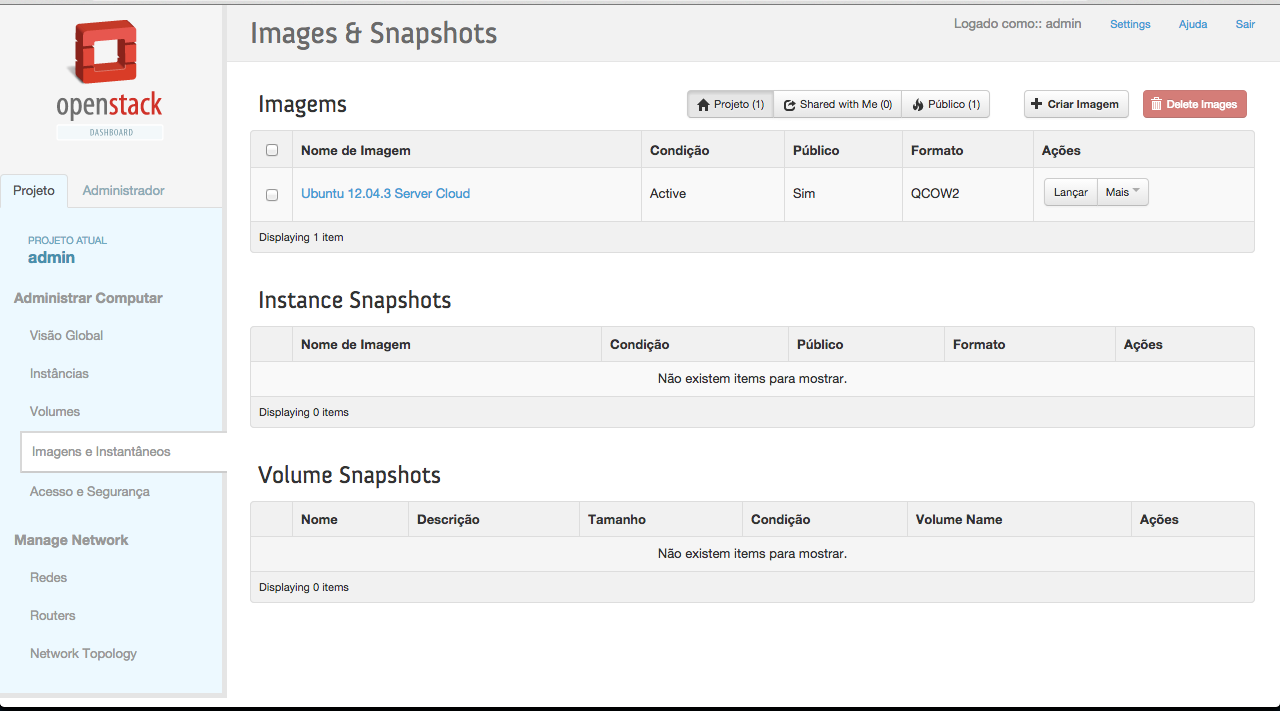
\includegraphics[scale=0.3]{imagem/imagens-e-snapshots.png}
  \caption{Interface para gerenciamento de volumes persistentes e snapshots}
  \label{img:imagens-e-snapshots}
\end{figure}

Existe também o controle de acesso e segurança das instância, onde são criados
usuários para o sistema. Cada usuário pode ter uma chave de criptografia, que será
usada para autenticá-lo com os servidores que tiver autorização de acesso e
fornecer um canal seguro de comunicação entre eles, como poder ser visto na
Figura \ref{img:acesso-e-seguranca-chaves}. Na área mostrada na Figura
\ref{img:acesso-e-seguranca-grupos-site} são
configuradas quais portas de cada servidor que aceitarão conexões de entrada.
Nesta seção, ilustrada pela Figura \ref{img:acesso-e-seguranca-acesso-api} é
possível também visualizar todos os pontos de acesso dos serviços
do \emph{cluster}, assim como as credenciais para acesso a eles.
Existe um \emph{super admin} capaz de utilizar esta interface para criar
\emph{tenants}\footnote{conceito utilizado para isolar dados de diferentes clientes
em um só sistema de uma maneira segura e eficiente}.
no \emph{OpenStack}, permitindo que diversas organizações utilizem o sistema sem
conhecimento e interferência entre si e com suas prórias regras individuais de
segurança.

\begin{figure}[h]
  \center
  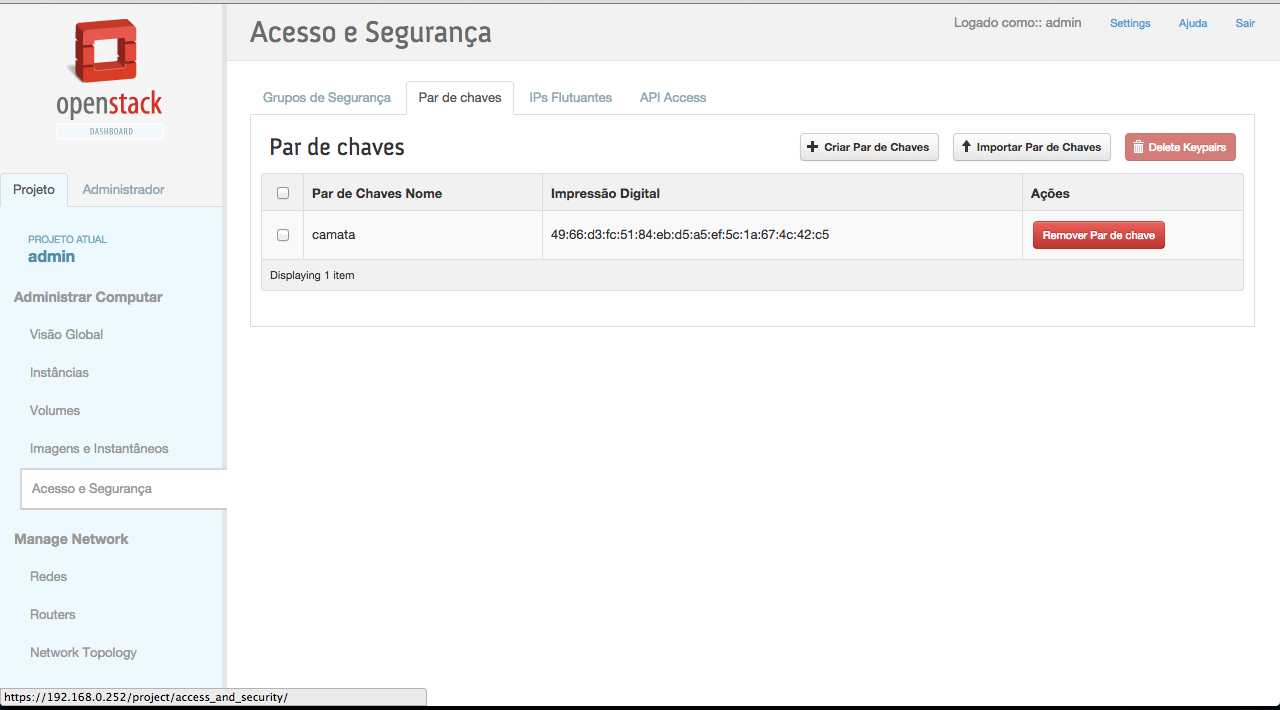
\includegraphics[scale=0.3]{imagem/acesso-e-seguranca-chaves.png}
  \caption{Interface para criação e visualização das chaves de acesso às máquinas
 virtuais}
  \label{img:acesso-e-seguranca-chaves}
\end{figure}

\begin{figure}[h]
  \center
  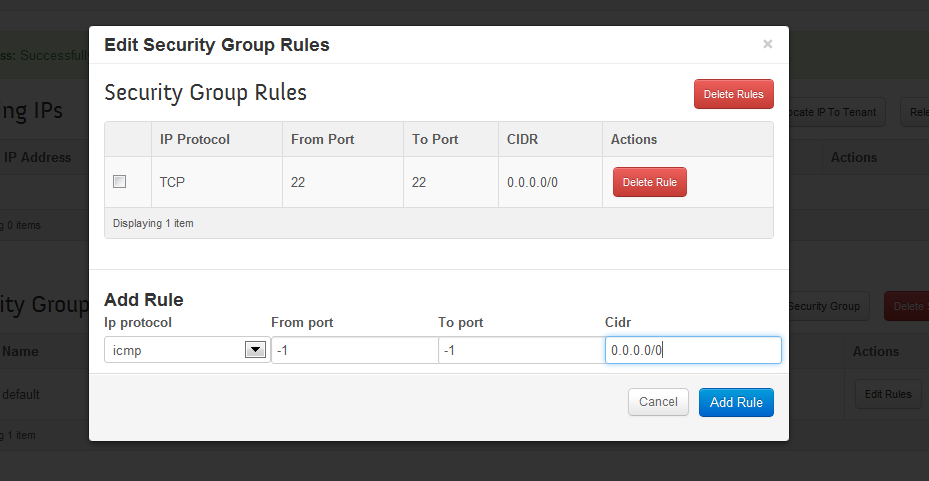
\includegraphics[scale=0.6]{imagem/acesso-e-seguranca-grupos-site.png}
  \caption{Configurações de permissões de rede de grupos}
  \label{img:acesso-e-seguranca-grupos-site}
\end{figure}

\begin{figure}[h]
  \center
  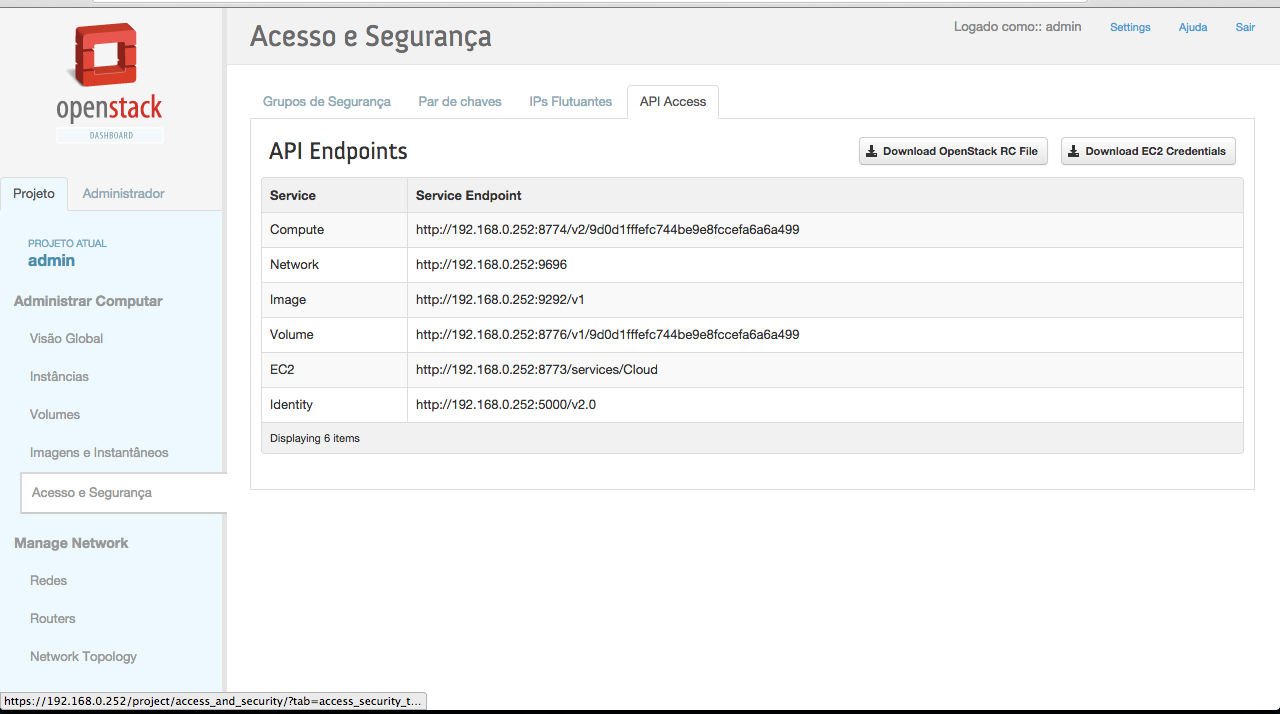
\includegraphics[scale=0.3]{imagem/acesso-e-seguranca-acesso-api.png}
  \caption{Visualização de \emph{URLs} de serviços e credenciais de acesso}
  \label{img:acesso-e-seguranca-acesso-api}
\end{figure}

Durante o desenvolvimento deste experimento, não havia uma ferramenta dentro do
\emph{OpenStack} para alcançar o nível de \emph{PaaS}: apenas ferramentas
desenvolvidas por terceiros (como o Juju, da Canonical, e o Tsuru, da Globo.com)
forneciam essa funcionalidade através das ricas APIs expostas pelo \emph{OpenStack}.
Contudo, antes mesmo do fim do experimento, foi desenvolvida e integrada uma
ferramenta para esta funcionalidade no projeto, chamada de \emph{Heat}, que não
foi considerada nesta análise devido à falta de tempo hábil.

Através de todas estas características, uma conclusão é eminente: o processo
de aquisição de infraestrutura computacional no paradigma de \emph{cloud computing}
é extremamente mais rápido e prático do que no modelo tradicional. Não bastante
esta vantagen, cada usuário pode se servir e adquirir a quantidade de recursos
necessários ao seu projeto e expandir ou diminuir conforme necessário (a interface
mostrada na figura \ref{img:criar-instancia-detalhes}, é também utilizada para a
edição das máquinas já criadas dentro do sistema. Além disso,
a interface é extremamente simples, possibilitando que qualquer pesquisador ou aluno
tenha acesso à infraestrutura que precisar para atingir seu objetivo, melhorando
ensino, pesquisa e também a própria universidade. Chegamos
então ao principal ponto econômico: graças a essa elasticidade, de uso e liberação
dos recursos, o \emph{cloud computing} oferece uma grande economia, evitando
o desperdício através de recursos escassos e fragmentados, favorecendo
ainda mais o melhoramento dos recursos computacionais da própria instituição.


% Também é um objetivo deste trabalho fazer uma
% discussão mais profunda sobre os detalhes técnicos da instalação
% do modelo, prover instruções para este processo, analisar as características do produto resultante
% e do processo, como um todo, verificar o nível do desenvolvimento do conjunto de ferramentas escolhido.
